%----------------------------------------------------------------------------
\chapter{A lekérdező program}\label{sect:Ellaboration}
%----------------------------------------------------------------------------
\section{Fejlesztés menetének áttekintése}
Első lépésként a bevezetőben megfogalmazott problémák megoldása érdekében, készítettem egy magas szintű lekérdező nyelvet az Essbase-hez, hogy a riport valamint az mdx nyelv összetevői alapján megfogalmaztam Xtextben egy metamodellt. Ezt a metamodellt az Xtend konkrét lekérdezések írásánál, fel tudja használni arra hogy validálja azt.

Ezek után az általam újonnan létrehozott nyelvbe, létrehoztam saját lekérdezést, amit futtatva, meg lehet nézni a havi kimutatást, költségeket.

Ezután készítettem egy szerkesztőt, amibe a fejlesztők tudnak dolgozni, ehhez egy Eclipse pugint csináltam, beépítve az Xtext nyelvtan elemző programomat. 

A program felhasználó kérésre transzformálja a megírt lekérdezést olyan Essbase lekérdezéssé amit az Essbase értelmezni tud, majd hálózaton elküldi a szervernek. A visszakapott objektumot ezután, a megfelelő parancsal meg lehet jeleníteni, riportolni, egy Latex pdf-be, amit a program generál.

 \begin{figure}[!ht]
\centering
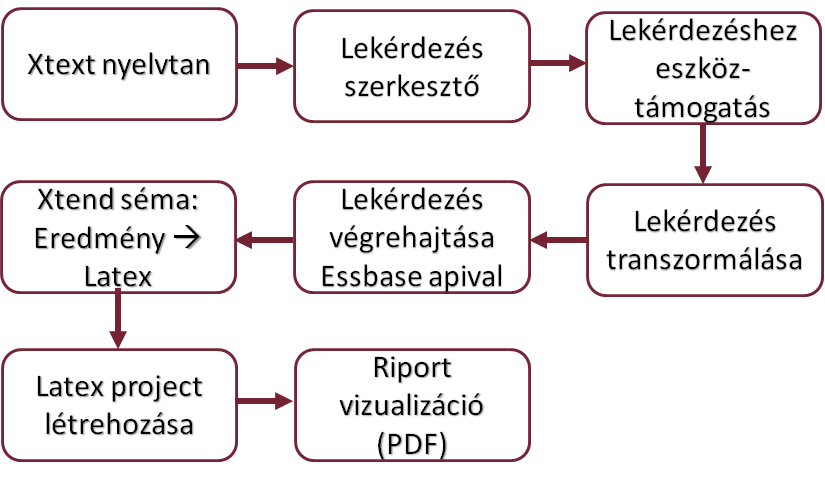
\includegraphics[width=120mm, keepaspectratio]{figures/overview.png}
\caption{A folyamat áttekintése} 
\label{fig:Overview}
\end{figure}

\begin{itemize}
  \item Xtext nyelvtan: Xtext metamodell elkészítése
  \item Lekérdezés szerkesztő: Eclipse fejlesztő környezetbe beépülő modul segítségével szerkesztő készítése
  \item Lekérdezéshez eszköz támogatás: Eclipse környezetből futtatjuk a lekérdezésünket
  \item Lekérdezés transzformálása: a program transzformálja a lekérdezést Essbase lekérdezéssé, és elkéri az adatokat a szervertől
  \item Xtend séma->Latex pdf: Xtend sémába beleteszi a program az Essbase szerver visszaadott adatait
  \item Latex projekt létrehozása: a program létrehozza a riport megjelenítésre szánt latex projektet
  \item Riport vizualizáció (PDF): végül kigenerálja a program a megfelelő diagrammokal a Latex pdf-et
\end{itemize}


\section{Lekérdező nyelv bemutatása}

Először is Xtextbe létrehoztam egy metamodelt, amibe definiáltam a saját riport lekérdezőmbe a valid parancsokat, amik kombinálják az MDX és a Riport parancsok lehetősgéeit, így mindkét nyelv lehetsőségeit lehet használni egy nyelvbe.

Jelenleg elkészült parancsok, amiket a metamodellezőbe már definiáltam.
\begin{itemize}
  \item $query ( param1, param2, param_n ):$ lekérdez az adatbázisból, a paraméterezésének megfelelően,
  gyakorlatilag egy referenciaként lehet használni, amit ezután ki lehet
  riportálni
  \item $dim:$ segítségével létrehozhatunk dimenzió referenciát, amivel ezután
  tudunk hivatkozni más parancsokban
  \item $group:$ segítségével létrehozhatunk group referenciát, amivel ezután
  tudunk hivatkozni más parancsokba
  \item $row:$ definiálhatjuk vele a sorokat, ami majd a kimeneti riportban meg
  fog jelenni, dim vagy group
  \item $link:$ meg lehet adni hogy a kimeneti riportban milyen szintig menjen le
  riport, meg lehet adni dimenziót, csoportot, vagy membert is
  \item $reportParameter:$ speciális paraméter megadására használható, amit a
  fejlesztő környezet felhasznál, és megjelenítést befolyásolja
  \item $report:$ bemenete egy query és futtatáskor a fejlesztő környezet generál
  egy pdf riportot 
\end{itemize}


\section{Validációs módszerek}
Az általam létrehozott új programozási nyelv tehát tudja validálni a megírt kódot már írás közben, egyszerre lehet riportokat és lekérdezéseket fejleszteni, elírások ellen véd a változó hivatkozás.

\section{Futtatás és a riport kimenete}
A megírt lekérdezést Eclipse-be lehet futtatni egy plugin segítségével a képernyőn látható módon:

\begin{figure}[!ht]
\centering
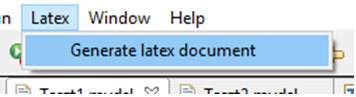
\includegraphics[width=60mm, keepaspectratio]{figures/run.png}
\caption{Riport futtatás Eclipse-ből} 
\label{fig:Overview}
\end{figure}

Majd amikor futtatjuk a lekérdezésünket a program generál egy latex projektet, egy Tex fájlal, amibe generálja a program az általunk megírt riport kimenetét:

 \begin{figure}[!ht]
\centering
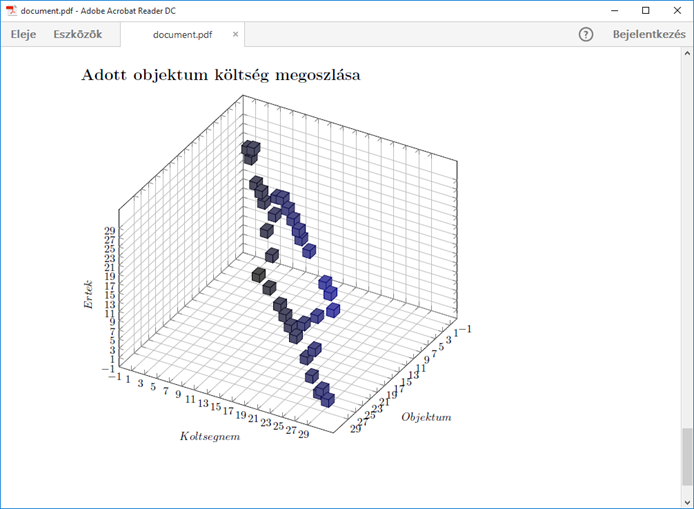
\includegraphics[width=120mm, keepaspectratio]{figures/Report.png}
\caption{Riport diagram példa} 
\label{fig:Overview}
\end{figure}





